% Filename: ForwardInverseToolkit.tex
% Last update: Thursday, September 7, 2017 by Ally Warner
%%%%%%%%%%%%%%%%%%%%%%%%%%%%%%%%%%%%%%%%%%%%%%%%%%%%%%%%%%%%%%%%%%%%%%

\section{Methods}
\label{sec:Methods}

%%Pipeline figure
\begin{figure}[H]
    \centering
    \includegraphics[width=\textwidth]{Figures/pipeline}
    \caption{Head/Brain Model Pipeline}
    \label{fig:pipeline}
\end{figure}

\subsection{Data Acquisition}
\label{sec:Data}

%%% Image and EEG Acquisitions 

To construct a high-resolution, personalized, anisotropic volume conductor whole-head model, $T_1$-, $T_2$- weighted, diffusion weighted, and functional magnetic resonance (MRI) scans were acquired on a healthy, female volunteer who is 23 years of age on a Skyra 3T full-body scanner (Siemens Medical Solutions, Erlangen, Germany). 

The $T_1$-weighted scan was performed with a 3D magnetization prepared rapid gradient echo (MPRAGE) sequence \cite{ref:mprage}. The parameters used were as follows: echo time: 3.41ms, repetition time: 2500ms, flip angle: 7 $^{\circ}$, resolution matrix size: 256x256 pixels, field of view: 256mm, 208 sagittal slices with a slice thickness of 1mm. Acquisition time was 10:42 minutes. 

The $T_2$-weighted scan was performed with a sampling prepared with application-optimized contrast using different flip angle evolutions (SPACE) sequence \cite{ref:space}. The parameters used were as follows: echo time: 406ms, repetition time: 3200ms, resolution matrix size: 256x256 pixels, field of view: 256mm, 208 sagittal slices with a slice thickness of 1mm. Acquisition time was 5:34 minutes. The subject did not move in between the two scans so the scans did not need to be registered. 

The diffusion weighted images (DWI) were acquired with multiband two-dimensional echo-planar imaging (EPI) \cite{ref:epi}. Both phase encoding directions were performed (anterior to posterior and posterior to anterior) with 64 diffusion directions each. Further sequence parameters for each scan was as follows: echo time: 76.8ms, repetition time: 4070ms, flip angle: 90 $^{\circ}$, resolution matrix size: 104x104 pixels, field of view: 208mm, 60 slices with 2.5mm slice thickness. Acquisition time was 5:05 minutes each. 

The function MRI (fMRI) scans were acquired with blood oxygenation level dependent contrast (BOLD). The following parameters were used:  echo time: 76.8ms, repetition time: 780ms, flip angle: 55 $^{\circ}$, resolution matrix size: 104x104 pixels, field of view: 210mm, 72 slices with 2mm slice thickness. Acquisition time was 10:32 minutes.

A continuous electroencephalogram (EEG) was recorded using a 256-channel HydroCel Geodesic Sensor Net that was connected to a NetAmps 400 amplifier and referenced online to a single vertex electrode shown in Figure \ref{fig:eegsetup}. Channel impedances were kept at or below 50 kOhms and signals were sampled at 250Hz. The EEG was recorded while the subject sat quietly in a chair, alternating two minute epochs of eyes open and eyes closed for a total of 12 minutes. 

All acquisition reports will be included with the dataset. 

%%EEG figure
\begin{figure}[!th]
    \centering
    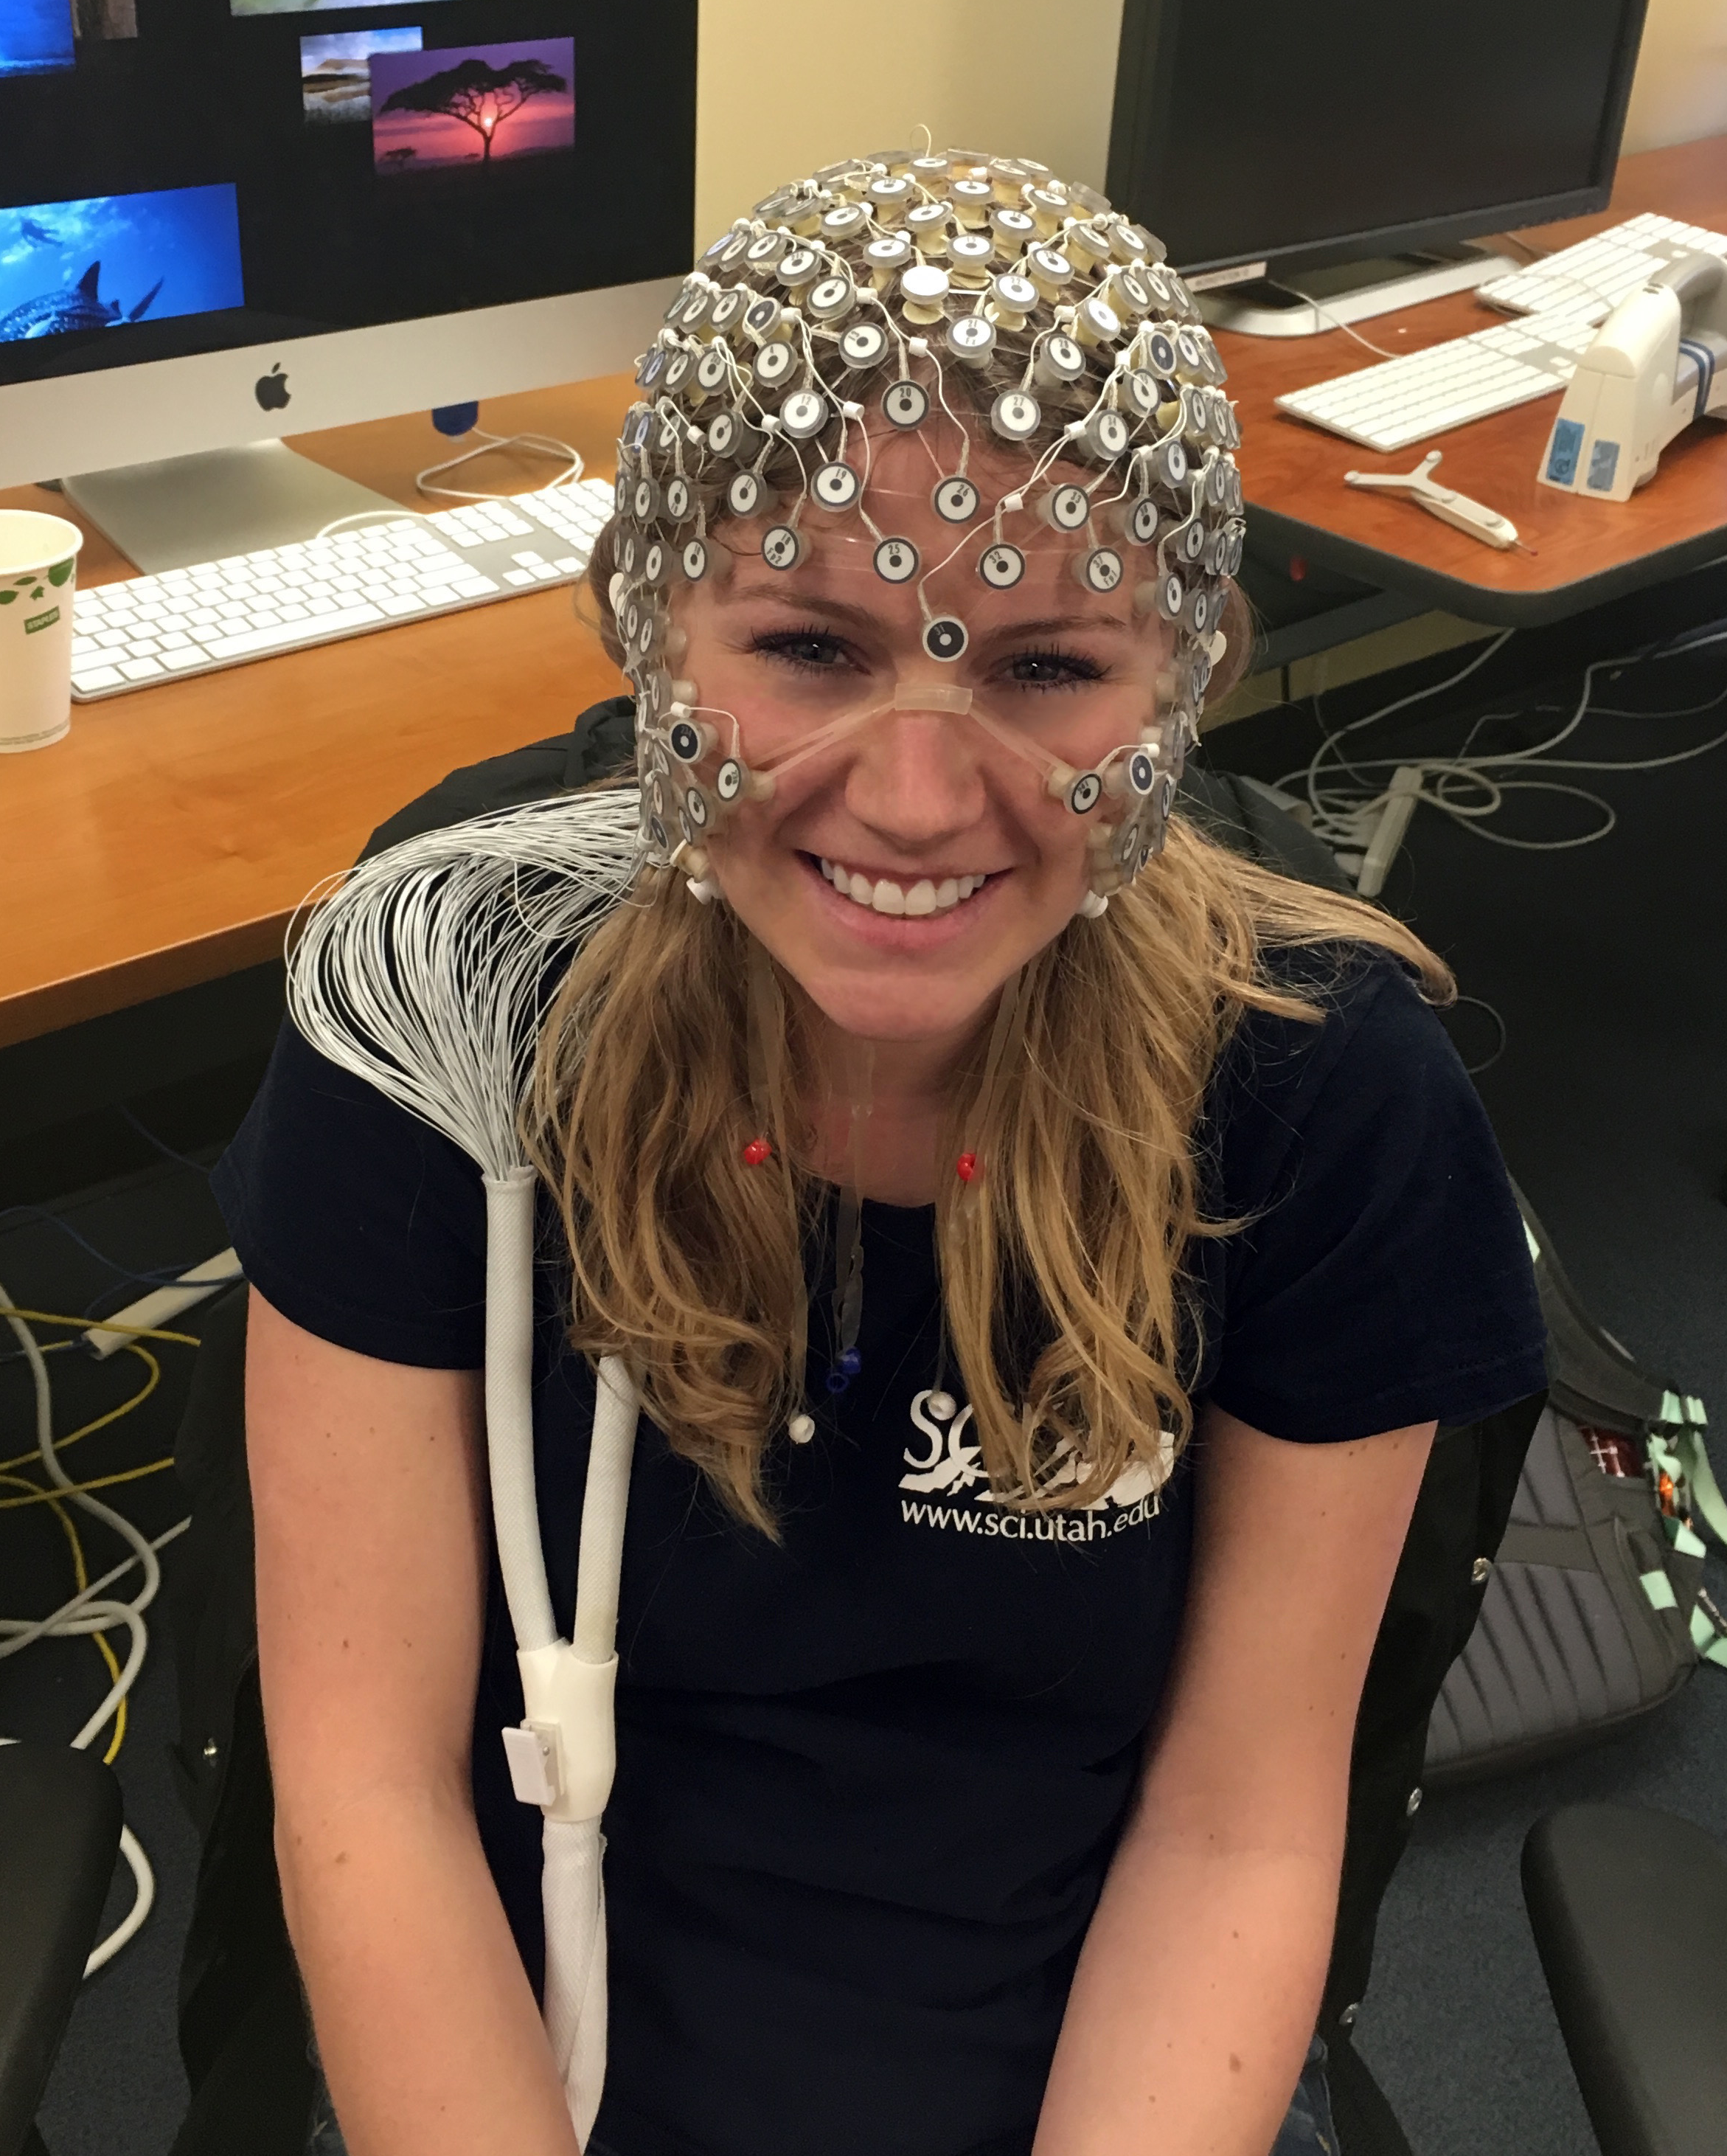
\includegraphics[width=7cm]{Figures/EEG_setup}
    \caption{256-channel HydroCel Geodesic Sensor Net on Subject}
    \label{fig:eegsetup}
\end{figure}

\subsection{Preprocessing of Images}
\label{sec:preprocess}

%FSL
\begin{wrapfigure}[16]{hr}{3cm}
    \centering
    \vspace{-35pt}
    \includegraphics[width=3cm]{Figures/FSL}
    \caption{FMRIB Software Library User Interface}
    \label{fig:fsl}
\end{wrapfigure}

\subsubsection{MRI Correction}

Bias field signal is a low-frequency, smooth signal that corrupts MRI images due to inhomogeneities in the magnetic fields of the MRI machine by blurring images reducing the high frequencies of the images such as edges and contours. It changes the intensity values of image pixels so that the same tissue has a different distribution of grayscale intensities across the image. \cite{ref:bias} An estimated bias field correction on the $T_1$ and $T_2$ MRI's was done using FMRIB Software Library (FSL) FAST \cite{ref:fslfast}, and will be further described in the Section \ref{sec:Seg}. Figure \ref{fig:fsl} shows FSL's basic user interface, which will be used multiple times throughout this pipeline. 

\subsubsection{DWI Distortion Correction}

Diffusion weighted images performed with EPI sequences are prone to distortions from rapid switching of diffusion weighting gradients, movement from the scanning table, and movement from the subject. The diffusion data was collected with reversed phase-encode blips (anterior to posterior (AP) and posterior to anterior(PA)), resulting in pairs of images with distortions going in opposite directions. From these pairs the susceptibility-induced off-resonance field was estimated using a method similar to that described in \cite{ref:fsltopup1} as implemented in FSL \cite{ref:fsltopup2} and the two images were combined into a single corrected one. This was accounted for using FSL's topup and eddy command line tools.

Before running these tools, an acquisition parameters text file needs to be created with the FSL-defined total readout time. 

\begin{figure}[H]
\centering
{\tt
\begin{varwidth}{\linewidth}
\begin{verbatim}
0  -1 0 0.0345
0   1 0 0.0345
\end{verbatim}
\end{varwidth}
}
\label{fig:acq}
\caption{Acquisition Parameters Text File}
\end{figure}

There are two parameters that are frequently needed when calculating and applying field maps: the effective echo spacing and the total readout time for an EPI sequence. ``Effective" echo spacing was used, rather than the actual echo spacing, in order to include the effects of parallel imaging, phase oversampling, etc. Multiplying this by the size of the reconstructed image in the phase direction will give you the reciprocal of the effective echo spacing:
\[
\text{Effective Echo Spacing (s) = 1/(BandwidthPerPixelPhaseEncode * MatrixSizePhase)}
\]

The total readout time (FSL definition) is:
\[
\text{Total readout time (FSL) = (MatrixSizePhase - 1) * EffectiveEchoSpacing}
\]

MRIConvert is a software package that provides all of the acquisition information about a dicom series, as well as converts to a NiFTI format, including effective echo spacing and total readout time \cite{ref:mriconvert}. To obtain this information, first load in the dicom series for either DWI acquisition. Choose ``Options" to ensure that the DWI will be saved as a NiFTI, and click ``Convert All." This will save all the files into the output directory specified upon opening MRIConvert. The text file will include the FSL-defined total readout time which should be contained in the acquisition parameter file in seconds. MRIConvert also outputs the b-values and b-vectors files, and they should be the same for both the DWI AP and DWI PA scans. The last input file needed is an ``index.txt" file. This text file contains one column with 65 rows (for 64 directions plus the b0 image) of 1's.

%MRIConvert
\begin{figure}[H]
    \centering
    \includegraphics[width=\textwidth]{Figures/combined}
    \caption{MRIConvert \textit{(left)} with Options \textit{(middle)} \& Output \textit{(right)} }
    \label{fig:mri_convert}
\end{figure}

Create a separate folder for topup results and include the following files: the acquisition parameters file, the index file, b-values, b-vectors, and the DWI AP and DWI PA files. In the following instructions, DWI AP was renamed as DWI\_up and DWIAP was renamed to DWI\_down. The b-values and b-vectors were renamed to dwi.bval and dwi.bvec, respectively. After all of these files are in place, run the following command line commands.

\lstdefinestyle{DOS}
{
    backgroundcolor=\color{white},
    basicstyle=\scriptsize\color{black}\ttfamily
}

\begin{lstlisting}[style=DOS]
fslroi DWI\_up b0\_up 0 1
fslroi DWI\_down b0\_down 0 1

fslmerge -t both\_b0 b0\_up b0\_down

topup --imain=both\_b0 --datain=acq_params.txt --config=mine.cnf --out=topup\_results
applytopup --imain=b0\_up,b0\_down --inindex=1,2 --datain=acq_params.txt
           --topup=topup\_results  --out=b0\_hifi

bet b0\_hifi b0\_hifi\_brain -m -f 0.2
eddy --imain=DWI\_up --mask=b0\_hifi\_brain\_mask --index=index.txt --acqp=acq_params.txt
     --bvecs=dwi.bvec --bvals=dwi.bval --fwhm=0 --topup=topup\_results --flm=quadratic
     --out=eddy\_unwarped

\end{lstlisting}

These commands first obtain the b0 image, which is the baseline image used for calculating field maps, for both encoding directions. Then the two b0's are merged together into one file. Topup and eddy are applied for distortion correction. Bet is applied for brain extraction. The distortion corrected file is named ``eddy\_unwarped.nii."

\subsubsection{Diffusion Tensor Images}

After the DWI images have been corrected, diffusion tensor images (DTI) are calculated using FSL's DTIFIT. Upon opening FSL choose ``FDT Diffusion." Then choose ``DTIFIT Reconstruct diffusion tensors" in the drop down menu, select to input files manually, and put in the files in Table \ref{dtifit}. (reference)

\begin{table}[H]
\centering
\caption{DTIFIT Input Files}
\label{ta:dtifit}
\begin{tabular}{|c|c|}
\hline
Diffusion weighted data: & eddy\_unwarmed.nii        \\ \hline
BET binary brain mask:   & b0\_hifi\_brain\_mask.nii \\ \hline
Output basename          & desired output location   \\ \hline
Gradient directions:     & dwi.bvec                  \\ \hline
b values:                & dwi.bval                  \\ \hline
\end{tabular}
\end{table}

DTIFIT will output the eigenvalues (named L1, L2, and L3) and the eigenvectors (named V1, V2, and V3) for the diffusion tensor field. The files were converted from NiFTI format to nrrd format using ITK-SNAP \cite{ref:itksnap} although there is a loss of precision. The files were then input into SCIRun to build the tensor field using the eigenvalue and eigenvectors. The SCIRun CalculateFieldData module only requires two eigenvectors as input because it calculates the third eigenvector automatically since it should be orthogonal to the first two. This process can be done in either SCIRun 4 or SCIRun 5 and the same results are produced. 

\begin{figure}[p]
\begin{center}
\includegraphics[width=\textwidth]{Figures/make_DTI.png}\\
\caption{SCIRun Network to Build Diffusion Tensor Data}
\label{fig:maketensornet}
\end{center}
\end{figure}

\begin{figure}[p]
\begin{center}
\includegraphics[width=0.75\textwidth]{Figures/DTI_1.png}
\includegraphics[width=0.75\textwidth]{Figures/DTI_2.png}
\caption{Diffusion Tensor Visualization}
\label{fig:tensorvis}
\end{center}
\end{figure}

The tensor field was built in SCIRun rather than in 3D Slicer \cite{ref:slicer} or FSL DTIFIT because the output data would be ``backwards" and couldn't be registered with the mesh. 

\subsubsection{fMRI}
\label{sec:fmripre}

fMRI data was preprocessed using the 1000 Functional Connectomes Project pipeline scripts (reference) which do anatomical preprocessing, functional preprocessing, registration to the $T_1$ MRI, segmentation, and nuisance signal regress. The outline pipeline used on this fMRI dataset, specific to the University of Utah, can be found at https://bitbucket.org/UtahBrainNetworks/base\_prep and includes specific instructions for installation, compilation, and usage.  

After running fMRI data through the pipeline ``rest.nii", the preprocessed fMRI file, was opened in Matlab using the ``load\_nii(`rest.nii')" function within the NiFTI toolbox \cite{ref:nifti}. The 4D ``img" variable (x, y, z, t) is then resized to a 2D variable (x*y*z,t) and saved to use in SCIRun. 
fre
\subsubsection{EEG}

The filetype of the EEG recordings in an .edf file after it had a 60Hz notch filter and its harmonics \cite{ref:filter}. The EEG signal matrix was obtained using a Matlab script called ``edfRead.m" \cite{ref:edfread}. To run this script use the following command ``[hdr, record] = edfread(fname)." The variable `record' will contain the signals. The last two rows of the matrix were removed because they did not correspond to EEG electrodes. Also the beginning and end of the experiment were cut out of the matrix when the EEG net is being put on and taken off. 

\subsubsection{Registration}

Since the subject did not move in between the $T_1$ and $T_2$ MRI, no registration was necessary before segmentation and meshing. The tetrahedral mesh was generated in its own coordinate space from the segmentation, and was registered to the DTI coordinate space with a rigid registration using SCIRun. The fMRI data was registered to the mesh coordinate space with a rigid registration using SCIRun. The fMRI data can use same transform to register to DTI later if desired. The SCIRun networks for registration are included in Section \ref{sec:sim}.

\begin{figure}[H]
\begin{center}
\includegraphics[width=.75\textwidth]{Figures/DTI_reg}
\caption{MRI to DTI Registration}
\label{fig:dtireg}
\end{center}
\end{figure}

\subsection{MRI Segmentation of Tissues}
\label{sec:Seg}

%%% Preparation for segmentation, trials, manual work 

Segmentation of the head tissues proved to be the most time consuming section of the pipeline. The head volume was segmented into air, cerebral spinal fluid (CSF), white matter, grey matter, skull, sinus, eyes, and scalp. Segmentation of the brain can be difficult due to the similar intensities of the different tissues, making merely applying a median filter and thresholding the image not enough. The majority of the segmentation work was done using Seg3D, a free volume segmentation and processing tool \cite{ref:seg3d}.

The brain was initially segmented by inputing a skull stripped $T_1$ MRI into FSL FAST Segmentation. This outputs CSF, white matter, and grey matter layers as well as a bias-corrected $T_1$ MRI. This method, compared with Freesurfer \cite{ref:freesurf}, Statistical Parametric Mapping through Matlab (SPM) \cite{ref:spm}, Atlas Based Classification through 3D Slicer \cite{ref:abc}, and Seg3D methods alone, produced the best initial brain segmentation results for this data due to how well it filled in each tissue. 
\begin{figure}[H]
    \centering
    \includegraphics[width=.8\textwidth]{Figures/FSL_FAST}
    \caption{FSL FAST User Interface }
    \label{fig:fslfast}
\end{figure}

\begin{figure}[H]
\begin{center}
\includegraphics[width=.32\textwidth]{Figures/FSLFAST_csf}
\includegraphics[width=.32\textwidth]{Figures/FSLFAST_wm}
\includegraphics[width=.32\textwidth]{Figures/FSLFAST_gm}
\caption{FSL FAST Output: CSF \textit{(left)}, White Matter \textit{(center)}, Grey Matter \textit{(right)}}
\label{fig:fastout}
\end{center}
\end{figure}

Although the FSL FAST results were a great improvement compared to the other segmentation trials, manual segmentation, completed with Seg3D, still needed to be done on those layers to add more detail and take out any cross over between the layers. Since white matter is the innermost layer, it was worked on first. First a threshold layer was created from the FSL FAST output. Every slice in every direction was inspected and manually edited whether that was adding more detail that could be seen with the naked eye or cleaning up noise from FSL FAST. This manual editing of the white matter took roughly 40 hours of work.

\begin{figure}[H]
\begin{center}
\includegraphics[width=.49\textwidth]{Figures/whitematter_before}
\includegraphics[width=.49\textwidth]{Figures/whitematter_after}
\caption{White Matter Segmentation: Before \textit{left} and After \textit{right} Manual Segmentation}
\label{fig:wm}
\end{center}
\end{figure}

After the white matter was completed, a threshold layer for grey matter was created from the FSL Fast output. Each slice in every direction of the grey matter was inspected as well. The white matter layer was removed from the grey matter using a boolean remove mask filter. Any holes between the two layers were decided manually. More detail was added to the grey matter folds to add to the CSF layer as well. The last part of editing the grey matter was decided to add a grey matter nucleus to the layer. The thresholding algorithms generated a lot of noise around these nuclei so they were segmented by hand, using the paintbrush tool, and added to the grey matter layer with a boolean or mask filter. The nuclei were also removed from the white matter layer using a boolean remove mask filter. The manual editing of the grey matter took roughly 20 hours of work.

\begin{figure}[H]
\begin{center}
\includegraphics[width=.49\textwidth]{Figures/greymatter_before_nuclei}
\includegraphics[width=.49\textwidth]{Figures/greymatter_added_nuclei}
\caption{Grey Matter Segmentation: Before \textit{left} and After \textit{right} Manual Segmentation. Grey matter nuclei were segmented manually.}
\label{fig:gm}
\end{center}
\end{figure}

After the grey and white matter layers were completed, the CSF layer was made by creating a solid threshold layer for the entire brain and removing the white and grey matter layers using a boolean remove mask filter. The white matter, grey matter, and CSF layers were then checked for holes, whether on the surface or the inside of the segmentation. Also a quality check on the layers was performed to ensure that the layers were at least two pixels wide. This is an important note for creating a hole-less tetrahedral mesh. The creation of the CSF layer and the manual editing and hole checking took roughly 4 hours of work.

\begin{figure}[H]
\begin{center}
\includegraphics[width=.49\textwidth]{Figures/CSF_seg}
\caption{CSF Segmentation}
\label{fig:csf}
\end{center}
\end{figure}

The skull and the sinus layers are the most difficult to segment using only an MRI because they both appear black in the image, and the volunteer did not have a computed tomography (CT) scan. The first attempt to create a bone layer was first to use FSL's skull stripping using the BET2 tool to create a skull. Then to threshold the remainder of the bones in Seg3D from the $T_1$ MRI and connect it to the skull from FSL. Although this gave a decent skull for only having an MRI layer, the method to segment sinus layer was still to be determined. As a second method, the skull was estimated from an MR-based synthetic pseudo-CT. An improved iterative version of the patch-based method was used described by Torrado-Carvajal et al. that takes the $T_1$ and $T_2$ images as input, and synthesize the pseudo-CT based on both images providing more refined and accurate bone boundaries \cite{ref:pseudoct}. 

\begin{figure}[H]
\begin{center}
\includegraphics[width=.75\textwidth]{Figures/pseudo_CT}
\caption{Pseudo-CT Scan}
\label{fig:ct}
\end{center}
\end{figure}

This method gave a good starting place for skull segmentation, but still needed manual editing. After using a median filter with one pixel radius and thresholding, each slice in each direction was manually edited by hand. Since the volunteer has a permanent retainer in their mouth, the mouth was segmented as solid bone for now. This is not concerning because the EEG cap used did not cover the volunteer's mouth. The pseduo-CT image also provided a segmentation of the sinuses and esophagus by thresholding the black pixels. After the thresholding, the sinus layer was also manually edited. Quality checks were done on both layers to ensure that there were no holes and that the layers were at least two pixels thick. Manually editing the second skull and the sinuses took roughly 30-40 hours of work. 

The eyes, skin, and air layers were simple, in comparison, to segment. The eyes were easily segmented by thresholding the $T_2$ MRI. The skin layer was segmented by thresholding the entire volume and removing all of the previous layers using a boolean remove mask filter. A quality check was performed on the skin layer to ensure that it was at least two pixels thick. The important places to check for this is at the bridge of the nose and the bottom of the chin. Last, the air was segmented by thresholding the entire image and removing the solid skin layer. There was a check to ensure that the segmentation did not contain any holes between layers after they were removed. To create these three layers took roughly 8 hours of work, most of which was ensuring there were no holes in the segmentation. This is imperative to creating a quality mesh.

\begin{table}[H]
\centering
\caption{Segmentation Time}
\label{tab:seg}
\begin{tabular}{|c|c|}
\hline
Segmented Tissue    & Amount of Work (hrs) \\ \hline
White Matter:       & 40                   \\ \hline
Grey Matter         & 20                   \\ \hline
CSF                 & 4                    \\ \hline
Skull and Sinus     & 35                   \\ \hline
Eyes, Scalp, \& Air & 8                    \\ \hline
\end{tabular}
\end{table}

\subsection{Finite Element Mesh Generation}
\label{sec:mesh}

%%% Settings for mesh generation, issues 

Segmentations were used to generate realistic three-dimensional geometries for use in subsequent finite element simulations. A smooth, linear, subject-specific, boundary-conforming, tetrahedral finite element mesh was generated using Cleaver software \cite{ref:cleaver} on a Late 2013 Mac Pro with a 2.7 Ghz 12 Core Intel Xeon E5 processor, 64 GB of RAM, and an AMD FirePro graphics card. Cleaver is a multimaterial meshing package that produces structured meshes of tetrahedral elements with guaranteed minimum element angles, resulting in quality meshes that require fewer computational resources. To make a very high resolution mesh with no holes the following parameters were used: 

\begin{table}[H]
\centering
\caption{Clever Settings (High Resolution)}
\label{my-label}
\begin{tabular}{|c|c|}
\hline
scaling factor:                    & 0.6                 \\ \hline
size multiplier:                   & 1.0                 \\ \hline
lipschitz:                         & 0.2                 \\ \hline
padding:                           & 0                   \\ \hline
element sizing method:             & adpative            \\ \hline
\end{tabular}
\end{table}

 Along with these parameters, indicator functions must be input to Cleaver. These are made by creating distance maps in Seg3D. Ensure the map is inverted before making the distance map. To reduce the size of the mesh, a mesh was made with a scaling factor of 1.0 with the remainder of the parameters as described before. The computing sizing field was exported from Cleaver and manipulated using SCIRun4 by changing how quickly the elements increase in size. This was done by multiplying the scaling by a factor of 27. The changed sizing field was then input into Cleaver with the same indicator functions and cleaved a new mesh.

\subsection{Mathematical Modeling}
\label{sec:math}

%%%MATH

The head mesh, with associated inhomogeneous and anisotropic regions, was used as a volume conductor to solve the following boundary value problem:
%
\begin{equation}
\label{eq:1} \nabla\cdot\sigma\nabla\Phi = -I_{V} \;\;\;\;\mbox{ in
}\Omega,
\end{equation} 
%
where $\Phi$ is the electrostatic potential, $\sigma$ is the electrical conductivity tensor, and $I_{V}$ is the current per unit volume defined within the solution domain, $\Omega$. Equation (\ref{eq:1}) is solved for $\Phi$ with a known description of $I_{V}$ and the Neumann boundary condition:
%
\begin{equation} \sigma\nabla\Phi\cdot{\bf
n} = 0\;\;\;\;\;\mbox{ on }\Gamma_{T}, 
\end{equation} 
%
which says that the normal component of the electric field is zero on the surface interfacing with air (here denoted by $\Gamma_{T}$). The brain and surrounding tissue and skull were discretized, and using dipoles for current source the electrical field was calculated within the brain and then projected onto the surface of the scalp. \cite{ref:math}

\subsubsection{Electrical Conductivity Preparation}
\label{sec:cond}

All electrical conductivities were homogeneous for each tissue with the exception of white matter when using tensor data. The isotropic conductivities are as follows \cite{ref:cond}: 

\begin{table}[H]
\centering
\caption{Isotropic Tissue Conductivity}
\label{tab:cond}
\begin{tabular}{|c|c|}
\hline
Tissue Type               & Isotropic Conductivity $(S/m)$ \\ \hline
White matter              & 0.1429                         \\ \hline
Grey Matter               & 0.3333                         \\ \hline
Cerebrospinal Fluid (CSF) & 1.79                           \\ \hline
Skull                     & 0.001                          \\ \hline
Skin                      & 0.4346                         \\ \hline
Sinus                     & 1e-6                           \\ \hline
Eyes                      & 0.5051                         \\ \hline
\end{tabular}
\end{table}

When DTI tensor data is added, there are two approaches to converting the tensor data to conductivities. The first is scaling the data \cite{ref:scaling}, and the second is giving the white matter a fixed ratio of conductivity. 

\begin{equation}
\sigma_{aniso} = \frac{\sigma_{iso}}{\sqrt[3]{d_1d_2d_3}}D
\end{equation}
where $D$ is the diffusion data, $d_i$ is the $i$th eigenvalue of $D$, and $\sigma_{iso}$ is the white matter isotropic conductivity.

\begin{equation}
\sigma_{aniso} = \begin{bmatrix}
v_1\\
v_2\\
v_3\\
W\\
\end{bmatrix}, 
W = \begin{bmatrix}
\sigma_{iso}\\
\frac{\sigma_{iso}}{10}\\
\frac{\sigma_{iso}}{10}\\
\end{bmatrix}
\end{equation}
where $v_i$ is the $i$th eigenvector of $D$ and $W$ is the white matter ratio vector and the ratio is $10:1$.

\subsubsection{Numerical Methods}
\label{sec:numerical}

%%% This paragraph addresses Finite Element Discretization

Solutions to Equation \ref{eq:1} were computed using finite element methods.  By applying 
Green's divergence theorem to Equation \ref{eq:1}, the following weak formulation is generated 
\begin{equation}
\int ((\bar{\sigma}_e + \bar{\sigma}_i)\nabla \phi_e) \cdot \nabla \psi(\bar{x})d\bar{x} = - \int (\bar{\sigma}
_i \nabla V_m)\cdot \nabla \psi(\bar{x})d\bar{x}, \quad \quad \forall \ \psi \in \Omega
\label{eq:galerkin}
\end{equation}
where, $\Omega$ is the linear, finite element mesh, $\psi$ represents the finite element basis functions characterized by local hat functions associated with mesh nodes. By applying this formulation to the finite dimensional mesh, we can reduce Equation \ref{eq:galerkin} to a system of linear equations 
\begin{equation}
A \phi_e = -RV_m
\label{eq:ReducedFormula}
\end{equation}
where $A$ and $R$ represent stiffness matrices defined by $A_{j,k} = \langle \nabla \psi_j,(\bar{\sigma}
_e + \bar{\sigma}_i)\nabla \psi_k \rangle_\Omega$ and $R_{j,k} = \langle \nabla \psi_j,\bar{\sigma}_i
\nabla \psi_k \rangle_\Omega$,
while $\phi_e$ and $V_m$ represent extracellular and transmembrane potentials, respectively.\cite{ref:fem}

%%% This paragraph addresses SCIRun as a solver
We used SCIRun, the open-source problem solving environment, to apply parameters and to solve Equation  \ref{eq:ReducedFormula} numerically.  Within the SCIRun environment, isotropic and anisotropic conductivity tensors were applied to the mesh as well as inhomogeneous regions, initial and boundary conditions were defined, and border regions were generated in order to compute potentials by way of a conjugate gradient method with a Jacobi preconditioner.

\subsection{Simulations \& Visualization}
\label{sec:sim}

All simulations and visualization were done in the SCIRun problem solving environment.

\subsubsection{Forward Problem}

When solving systems described in Section \ref {sec:math} from a known source to the EEG electrodes, it is called a forward problem. To solve the opposite is to solve an inverse problem and would usually be the case for finding sources for subjects with neurological disorders. In this project, we have set up SCIRun networks to solve forward problems with known sources and to write a lead field matrix for inverse problem networks made in the future. We solve the forward problem with an isotropic system and an anisotropic system, which includes DTI data. 

For the isotropic case necessary inputs are the tetrahedral head mesh, isotropic conductivities, the head segmentation, the physical electrode locations, and dipole sources. The physical electrode locations and dipole sources were part of the EEG dataset. The electrodes have the fiducials removed and the only dipole sources that are used are those that the user chooses. There are 4800 dipoles in the data set and there should be 256 electrodes after the fiducials are removed. The head mesh was registered to the head segmentation with a rigid registration and after the flat tets are cut out the conductivities are mapped to their respective tissues. The electrodes and dipoles are registered to the head mesh with the same transform. The system is solved with the mapped data and the chosen dipole sources. The solution is then mapped onto the mesh and the electrodes for visualization. Streamlines and isolines are also included in the visualization.

For the anisotropic case, the network is going to be largely the same with the exception of the diffusion tensor data set used as white matter conductivities after it was scaled as explained in Section \ref{sec:cond} and the DTI to mesh transform is needed as input. The head mesh, electrodes, and dipoles were registered to the DTI space with a rigid registration and the head segmentation wasn't needed.

\begin{figure}[p]
\begin{center}
\includegraphics[width=\textwidth]{Figures/iso_network.png}\\
\caption{SCIRun Network for Isotropic Forward Problem}
\label{fig:isofor}
\end{center}
\end{figure}

\begin{figure}[p]
\begin{center}
\includegraphics[width=\textwidth]{Figures/aniso_network.png}\\
\caption{SCIRun Network for Anisotropic Forward Problem}
\label{fig:anisofor}
\end{center}
\end{figure}

\begin{figure}[p]
\begin{center}
\includegraphics[width=\textwidth]{Figures/fmri_network.png}\\
\caption{SCIRun Network for fMRI Visualization}
\label{fig:fmrivis}
\end{center}
\end{figure}

\begin{figure}[p]
\begin{center}
\includegraphics[width=\textwidth]{Figures/EEG_network.png}\\
\caption{SCIRun Network for EEG Visualization}
\label{fig:eegvis}
\end{center}
\end{figure} 

\subsubsection{fMRI}

The fMRI data is visualized one step at a time using the 2D matrix described in Section \ref{sec:fmripre} as input and viewing one column at a time. Each column is set onto a lattice volume, which is then rotated 180 degrees, smoothed, thresholded and clipped for easier rigid registration. The fMRI is registered to the tetrahedral mesh using the bounding boxes and manual registration. After registration, the smoothed fMRI data is mapped onto the mesh using a mapping matrix with a linear interpolation basis. 

\subsubsection{EEG}

We visualized the EEG data on the physical electrode locations. These were registered to the mesh space with a rigid registration after the fiducials were removed from the electrode data set. The filtered and cut EEG matrix was used as input and each time step was represented as a column. The electrodes were then placed onto the mesh, and EEG data mapped onto the electrodes one time step at a time. 
